\subsection{Misure di temperatura}

\begin{wrapfigure}[14]{l}{0.45\textwidth}
\centering
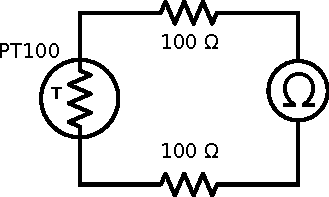
\includegraphics[width=.25\textwidth]{../E05/latex/c_PT100_2wire.pdf}
\caption{Circuito di controllo della temperatura a distanza: PT100 è il termoresistore al platino, l'ohmetro misura la resistenza in funzione della temperatura e le due resistenze da \SI{10}{\ohm} simulano i cavi lunghi.}
\label{cir5:2wire}
\end{wrapfigure}

Nell'ultima parte dell'esperienza abbiamo eseguito misure di temperatura utilizzando una termoresistenza al platino PT100.
Essa non è altro che una resistenza di cui sono noti con sufficiente precisione alcuni parametri: il valore ad una data temperatura e il coefficiente di temperatura $\alpha$.

Sapendo che il valore di resistenza è dipendente dalla resistività elettrica del materiale $\rho$ che a sua volta dipende dalla temperatura (nel caso di metalli), secondo le seguenti relazioni:
	$$	R = \frac{\rho L}{S}
			\qquad \qquad
		\rho = \rho_0 \left[ 1 + \alpha \left( T - T_0 \right) \right]$$
dove L è la lunghezza del materiale e S la sezione, mentre $\rho$ dipende dalla resistività $\rho_0$ alla temperatura di riferimento $T_0$ e dal coefficiente di temperatura $\alpha$.
Combinando le due equazioni precedenti si ottiene la dipendenza del valore di resistenza dalla temperatura:
\begin{equation}
R = R_0 \left[ 1 + \alpha \left( T - T_0 \right) \right]
\end{equation}

\begin{wrapfigure}[17]{r}{0.45\textwidth}
\centering
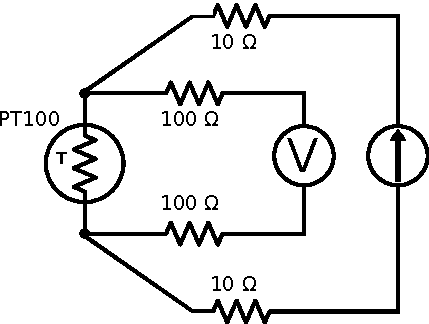
\includegraphics[width=.3\textwidth]{../E05/latex/c_PT100_4wire.pdf}
\caption{Configurazione di misura a quattro fili: nella maglia esterna scorre la corrente data dal generatore mentre nella maglia interna non scorre corrente. Il voltmetro ha un'impedenza idealmente infinita.}
\label{cir5:4wire}
\end{wrapfigure}

Invertendo la formula si ottiene:
\begin{equation}
T = T_0 + \frac{1}{\alpha}\left( \frac{R}{R_0}-1 \right)
\end{equation}
Nel nostro caso il costruttore ci ha fornito i dati relativi alla temperatura di riferimento $T_0 =$ \SI{0}{\degreeCelsius}:
$$R_0 = \SI{100}{\ohm} \quad \quad \alpha = \SI[per-mode=symbol]{0.3850}{\ohm\per\degreeCelsius}$$

Conoscendo il comportamento della termoresistenza abbiamo simulato il caso in cui si volesse controllare la temperatura di un laboratorio a distanza.
I circuito che simulava questa situazione è riportato in Figura \ref{cir5:2wire}

Abbiamo notato subito che le misure ricavate con questo circuito soffrivano dell'errore sistematico dato dalle resistenze in serie da \SI{10}{\ohm}.
Infatti il valore di resistenza letto dall'ohmetro era di \SI{130}{\ohm}, che dava in risultato una temperatura ambiente di $\approx$ \SI{78}{\degreeCelsius}, evidentemente errata.

Per evitare questo tipo di problemi abbiamo effettuato una misura a quattro fili.
In questa modalità il multimetro funzionava come generatore di corrente costante tramite due boccole e da voltmetro con le altre due boccole utilizzate.
Lo schema riportato in Figura \ref{cir5:4wire} mostra come la misura questa volta sia effettuata acquisendo la differenza di potenziale ai capi della termoresistenza data dalla corrente del generatore.
In questa configurazione non vi è l'errore sistematico della misura a due fili, in quanto grazie all'alta impedenza del voltmetro, nella maglia interna non scorre corrente e pertanto ai capi delle resistenze su tale maglia non vi è alcuna caduta di potenziale.

Nella tabella seguente sono riportati i valori per $T_0 =$ 0, per due temperature vicine alla temperatura ambiente, per una temperatura ottenuta raffreddando con una bomboletta di refrigerante e riscaldando il termoresistore a temperatura corporea.

\begin{center}
{\renewcommand{\arraystretch}{1.4}%
\begin{tabular}{c|c c c c c}
$R$ [\si{\ohm}] 		& $R_0 =$ 100 	& 110.24 & 111.32 & 83.37 & 114.71\\ 
\hline 
$T$ [\si{\degreeCelsius}] 	& $T_0 =$ 0 	& 26.6 & 29.4 & -43.2 & 38.2 \\ 
\end{tabular}}
\end{center}